%%%%%%%%%%%%%%%%%%%%%%%%%%%%%%%%%%%%%%%%%
% Simple Sectioned Essay Template
% LaTeX Template
%
% This template has been downloaded from:
% http://www.latextemplates.com
%
% Note:
% The \lipsum[#] commands throughout this template generate dummy text
% to fill the template out. These commands should all be removed when 
% writing essay content.
%
%%%%%%%%%%%%%%%%%%%%%%%%%%%%%%%%%%%%%%%%%

%----------------------------------------------------------------------------------------
%	PACKAGES AND OTHER DOCUMENT CONFIGURATIONS
%----------------------------------------------------------------------------------------
%
\documentclass[12pt]{article} % Default font size is 12pt, it can be changed here
\pagestyle{empty} % entfernt die Seitenzahlen

\renewcommand{\familydefault}{\sfdefault} % Standardfont ändern auf Sans Serif (bny)

\usepackage[left=2cm,right=2cm,top=1.5cm,bottom=1.5cm]{geometry} % Required to change the page size to A4
% manuelle Seitenränder eingesetzt durch bny einfach alles inkl. [] wieder löschen, 09.04.2016
\geometry{a4paper} % Set the page size to be A4 as opposed to the default US Letter

\usepackage[utf8x]{inputenc}
\usepackage[german]{babel} % Sprache umschalten /hat funktioniert bis auf Authors, bny 13.04.2016
\usepackage{graphicx} % Required for including pictures
\usepackage{graphics} % Möglichkeit Bilder im Textfluss einzubinden - bny / 09.04.2016
\usepackage{float} % Allows putting an [H] in \begin{figure} to specify the exact location of the figure
\usepackage{wrapfig} % Allows in-line images such as the example fish picture
\usepackage[dvipsnames]{xcolor} % von bny hinzugefügt
\usepackage{paralist} % Aufzählung mit weniger Abstand - bny
\usepackage[bookmarksopen=true,colorlinks,linkcolor = black]{hyperref} % Hinzugefügt am 21.04.2016 - bny
\usepackage{adjustbox} % Bild/Text ausrichten; hinzugefügt am 21.04.2016, bny

\linespread{1.2} % Line spacing

%\setlength\parindent{0pt} % Uncomment to remove all indentation from paragraphs

\graphicspath{{Pictures/}} % Specifies the directory where pictures are stored

\setlength{\parindent}{0pt} % Neue Absätze nicht einrücken - bny 09.04.2016

\newcommand{\HRule}{\rule{\linewidth}{0.5mm}} % Defines a new command for the horizontal lines, change thickness here


\newcommand{\col}[1]{\textbf{\textcolor[rgb]{0.4392157,0.1882353,0.627451}{#1}}}


%%%----------------------------------------------------------------------------------------
%%%	BEGIN DOCUMENT
%%%----------------------------------------------------------------------------------------

\begin{document}

%%%----------------------------------------------------------------------------------------
%%%	TITLE PAGE
%%%----------------------------------------------------------------------------------------

% \begin{titlepage}

%%% \textsc{\LARGE Emch & Berger }\\[1.5cm] % Name of your university/college

% \begin{figure}[t] % Example image
% \flushright  % rechtsbuendig
% 
\includegraphics[width=0.2\linewidth]{0_EmBeLogo}
%%% \caption{Das Menü in CUBE PA}
%%% \label{fig:speciation}
% \end{figure}

% \vspace*{6cm}

% \center % Center everything on the page

% \HRule \\[0.4cm]
% { \huge \bfseries CUBE ProjectAssistant}\\[0.4cm] % Title of your document
% \HRule \\[1.5cm]

% \textsf{\Large Benutzerhandbuch}\\[0.5cm] % Major heading such as course name
% \textsf{\large Version 2.11 / 10.07.2018}\\[0.5cm] % Minor heading such as course title


% \pagebreak
% \vspace*{15cm}

% \flushleft\textbf{ Impressum}
% \rule{\textwidth}{1pt}

% \begin{tabular}{lp{12cm}}
% Auftragsnummer & BE.N.\\
% Auftraggeber & .\\
% Datum & 10.07.2018\\
% Version & 2.11\\
% Autoren & Dieter Schopfer, Benjamin Nyffenegger, Rayane Zahreddine, Adrian Johner, Markus Schafroth, Simon Heimberg\\
% Freigabe & Markus Schafroth\\
% Verteilen & .\\
% Datei & .\\
% Seitenzahl & 180\\
% Copyright & \copyright{ Emch+Berger AG Bern}\\
% \end{tabular}

% \vfill % Fill the rest of the page with whitespace

% \end{titlepage}

%%%----------------------------------------------------------------------------------------
%%%	TABLE OF CONTENTS
%%%----------------------------------------------------------------------------------------

% \tableofcontents % Include a table of contents

% \newpage % Begins the essay on a new page instead of on the same page as the table of contents 

%%%----------------------------------------------------------------------------------------
%%%	Eingebundene Kapitel
%%%----------------------------------------------------------------------------------------

\section{Upgrade-Info CUBE Project Assistant} % Major section
% Example citation \cite{Figueredo:2009dg}. (Literaturangabe; Literaturliste)

Ihre CUBE Project Assistant-Instanz wird auf die Version 2.12 aktualisiert. Wir führen neue Funktionen ein. Gleichzeitig werden einige Funktionen angepasst. Um den Umstieg reibungslos zu gestalten, sind die wichtigsten Änderungen untenstehend beschrieben.

\subsection{Dokumente hochladen}
In verschiedenen Modulen können nicht nur Dokumente verknüpft, sondern neue Dokumente hochgeladen werden. Zum einen wird damit die Dokumentenverknüpfung (z.B. Sitzungsbeilage) erstellt, zum anderen steht das hochgeladen Dokument in der Dokumentenablage ebenfalls zur Verfügung.

\begin{figure}[H]
\center{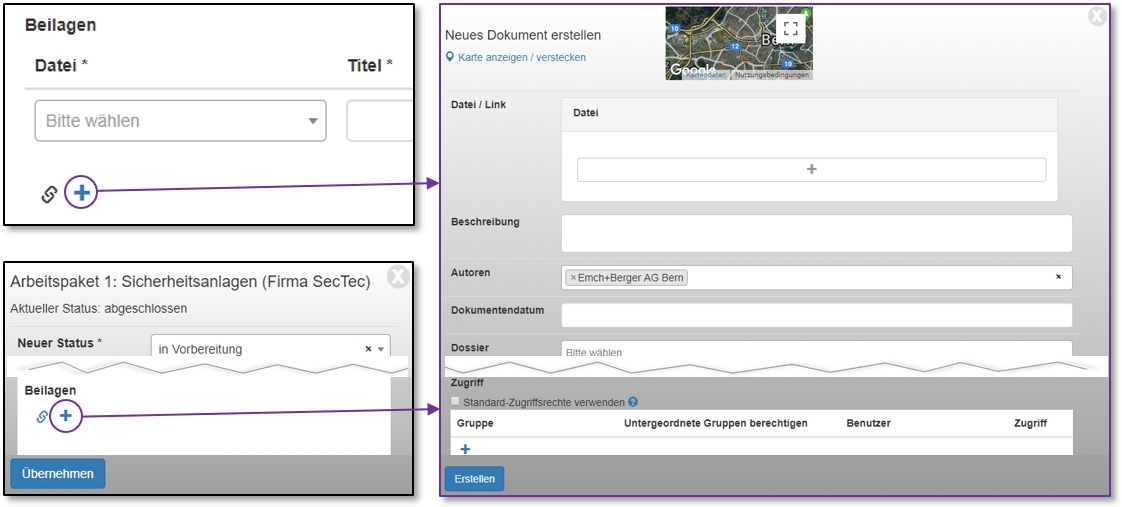
\includegraphics[width=1\linewidth]{../chapters/01_generisch/pictures/FileUpload.jpg}}
% \caption{Neue Sitzung erfassen}
% \label{fig:speciation}
\end{figure}

Klicken Sie jeweils auf das Pluszeichen 
\includegraphics[height=12pt]{/Icons/Pluszeichen.jpg}, wird ein zusätzliches Fenster geöffnet. Wie in der Dokumentenablage lassen sich nun weitere Angaben zum Dokument hinzufügen.

\subsection{Dokumente per Link versenden}
Dokumente können in Emails als Attachement oder mit sicherem Link versendet werden.

\begin{figure}[H]
\center{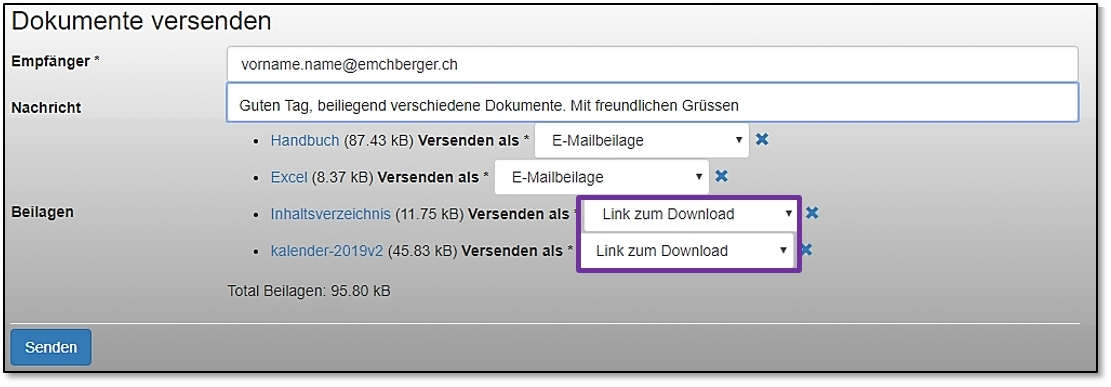
\includegraphics[width=1\linewidth]{../chapters/01_generisch/pictures/EmailLink.jpg}}
% \caption{Neue Sitzung erfassen}
% \label{fig:speciation}
\end{figure}

Bei der Auswahl 'Link zum Download' wird eine sichere Verbindung zu CUBE PA erstellt. Der Empfänger muss sich für das Herunterladen des Dokuments bei CUBE PA nicht anmelden. Dieser sichere 'Link' hat eine Gültigkeitsdauer von 30 Tagen und läuft danach automatisch ab.

\subsection{Datensätze in der Übersicht bearbeiten}
In der Adressliste wie auch in den Pendenzen können die gewünschten Änderungen gerade in der Übersicht vorgenommen werden:

\begin{figure}[H]
\center{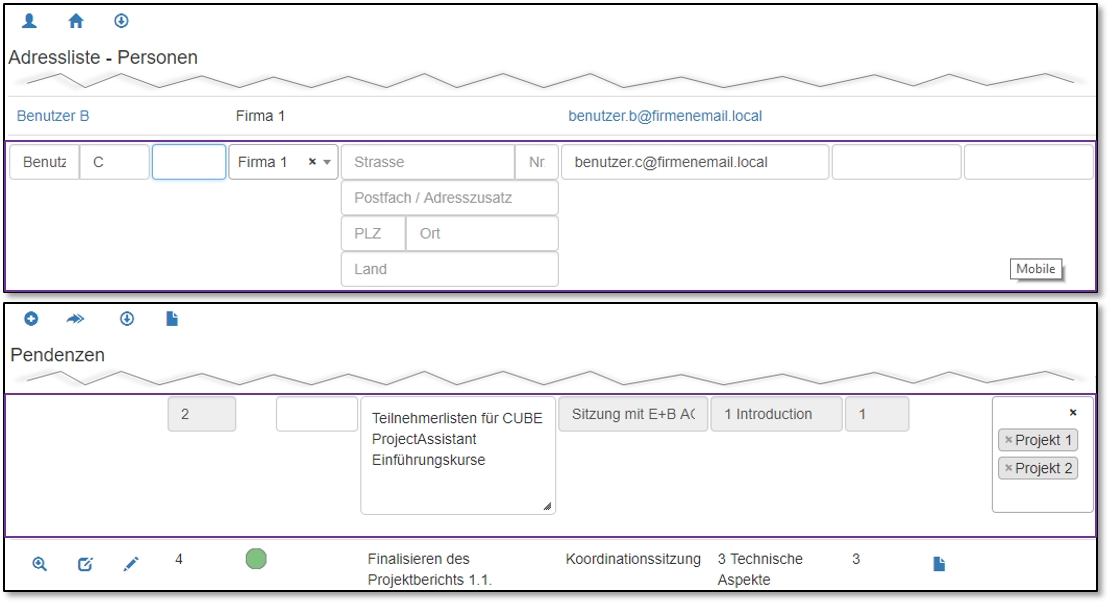
\includegraphics[width=1\linewidth]{../chapters/01_generisch/pictures/InlineEdit.jpg}}
% \caption{Neue Sitzung erfassen}
% \label{fig:speciation}
\end{figure}

\textbf{Einige Features:}
\begin{compactitem}
	\item Mit Doppelklick in einen Datensatz wird dieser für die Bearbeitung geöffnet
	\item Erneuter Doppelklick speichert die Daten und schliesst die Bearbeitung
	\item Ist bereits ein Datensatz für die Bearbeitung geöffnet, kann kein zweiter geöffnet werden (Meldung erscheint)
	\item Ist eine Geschäftsadresse hinterlegt, wird diese mit entsprechendem Vermerk angezeigt. Wird eine separate Adresse hinterlegt, hat diese Priorität - wird sie wieder gelöscht, erscheint erneut die Geschäftsadresse
	\item Mit Klick auf den Stift erreichen Sie die gleiche Funktion wie mit Doppelklick in den Datensatz
	\item Sie können mit Klick auf das Bearbeitungssymbol 
\includegraphics[height=12pt]{/Icons/Bearbeiten.jpg} auch die Formularseite öffnen und Änderungen vornehmen.
\end{compactitem}

\vspace{\baselineskip}

\textbf{Tipp:} Neu haben Sie jeweils oben in der Bildmitte zwei Schaltflächen: 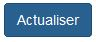
\includegraphics[height=14pt]{/Icons/B_Uebernehmen.jpg} und 
\includegraphics[height=14pt]{/Icons/ueb_schliessen.png}. Mit Klick auf 
\includegraphics[height=14pt]{/Icons/ueb_schliessen.png} gelangen Sie in der Regel auf die Übersichtsseite.

\vspace{\baselineskip}

Auf YouTube finden Sie verschiedene Tutorial-Videos, welche Ihnen weitere hilfreiche Unterstützung für die Arbeit mit CUBE Project Assistant bieten \href{https://www.youtube.com/channel/UCYWA8nERo4vTPYWP0WJ32hw}{\color{blue}[Link]}.

\vspace{\baselineskip}

Die Detailbeschreibungen zu obigen Funktionen finden Sie im CUBE PA-Benutzerhandbuch. Für weitere Fragen kontaktieren Sie uns unter {\color{red} cube.support@emchberger.ch}.

\section{Upgrade-Info CUBE PA - Pilatus} % Major section
% Example citation \cite{Figueredo:2009dg}. (Literaturangabe; Literaturliste)

Ihre CUBE ProjectAssistant-Instanz wird in Kürze von der Version 2.7 auf die Version 2.11 aktualisiert.

\vspace{\baselineskip}

Wir führen mit dieser Instanz viele neue Funktionen ein. Gleichzeitig werden einige Funktionen angepasst. Um den Umstieg reibungslos zu gestalten, sind die wichtigsten Änderungen untenstehend beschrieben.

\subsection{Änderungen bei der Dokumentenablage} % Sub-section

In der Übersicht der Dokumentenablage ist die Tagstruktur-Navigation gleich geblieben:

\begin{figure}[H]
\center{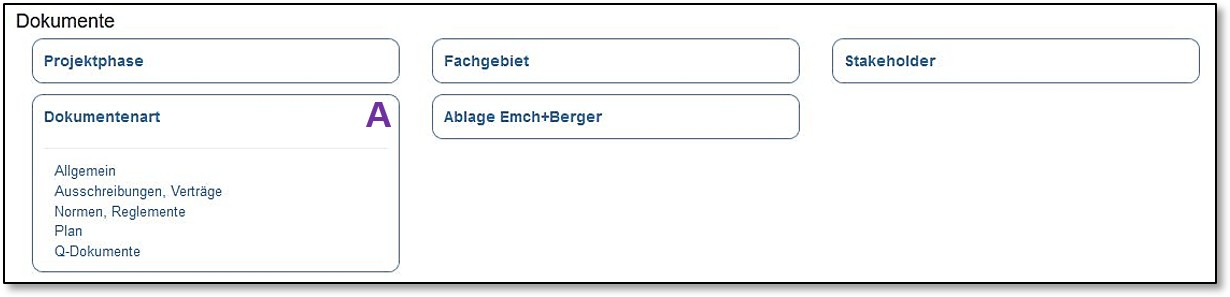
\includegraphics[width=1\linewidth]{../chapters/02_Pilatus/pictures/01_Dok_Overview_cut.jpg}}
% \caption{Neue Sitzung erfassen}
% \label{fig:speciation}
\end{figure}

Sie können wie gewohnt nach den Tags filtern oder via Navigationsbox die Tags suchen und auswählen \col{(A)}.

Im Bearbeitungsmodus (
\includegraphics[height=12pt]{/Icons/bearbeiten.jpg}) wurde die Handhabung mit den Tags in der Version 2.11 überarbeitet und bietet eine übersichtlichere Auswahl der Tags:

\begin{figure}[H]
\center{
\includegraphics[width=1\linewidth]{../chapters/02_Pilatus/pictures/02_Dok_Edit_cut.jpg}}
% \caption{Neue Sitzung erfassen}
% \label{fig:speciation}
\end{figure}

Neu finden Sie  den Button 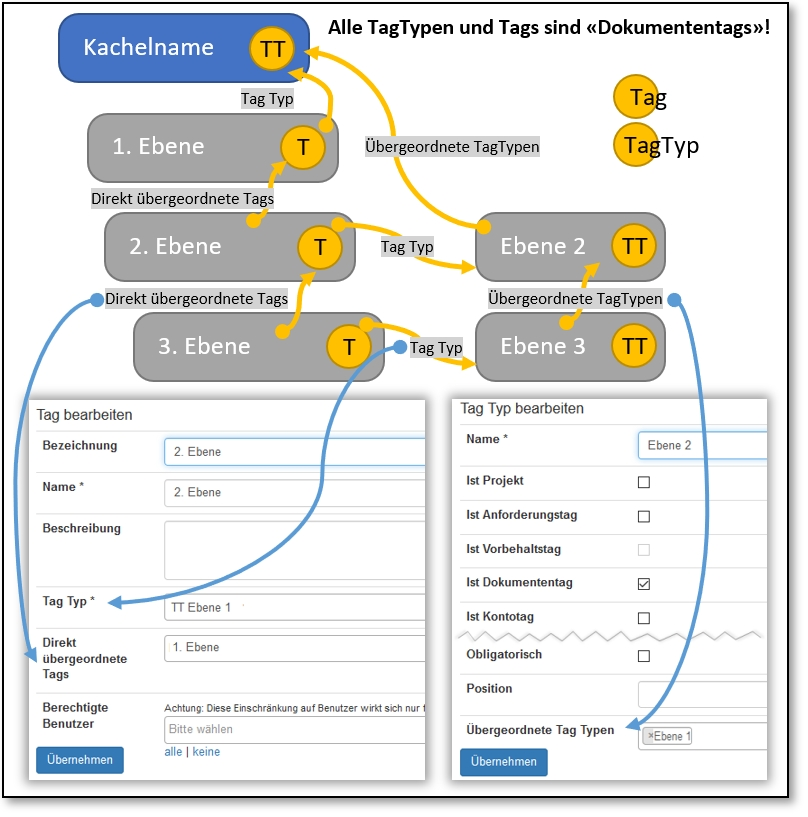
\includegraphics[height=12pt]{/Icons/Tagstruktur.jpg} \col{(B)}, mit welchem Sie direkt die neue Navigation der Tags aufrufen:

% \pagebreak

\begin{wrapfigure}[11]{l}{6.5cm}   % [x] Wie manche Zeile soll sich um die Grafik "brechen"
  \vspace{-23pt}      % Grundwert war 20; mit 30 schön oben beim Text ausgerichtet
  \begin{center}
    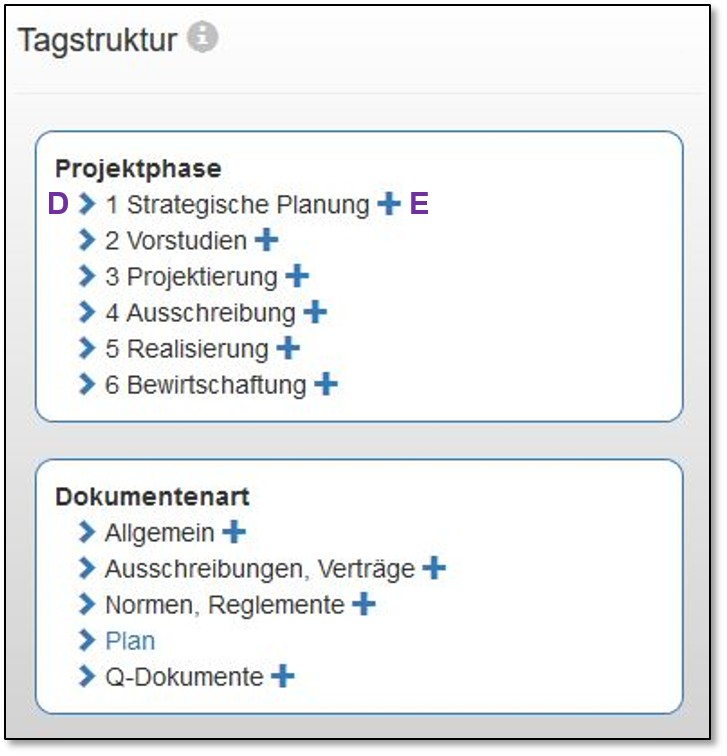
\includegraphics[width=1\linewidth]{../chapters/02_Pilatus/pictures/04_Dok_Struktur_eingeklappt.jpg}
  \end{center}
  \vspace{-20pt}
%  \caption{Das Menü verwenden}
  \vspace{-10pt}
\end{wrapfigure}

\textbf{Anwendung}: Navigieren Sie mit 
\includegraphics[height=12pt]{/Icons/Pfeil_rechts.jpg} \col{(D)} und klicken Sie hinter dem gesuchten Tag auf das 
\includegraphics[height=12pt]{/Icons/Pluszeichen.jpg}-Zeichen \col{(E)} (Mehrauswahl von Tags ist möglich) und schliessen Sie das Tag-Fenster oben rechts mit 
\includegraphics[height=12pt]{/Icons/X_Button.jpg}. Die Tags wurden im Feld Tags übernommen und können dort auch wieder gelöscht werden.

\vspace{\baselineskip}

\textbf{Hinweis}: Wenn Sie auf der Bearbeitungsseite (
\includegraphics[height=12pt]{/Icons/bearbeiten.jpg}) unter Tags Stichworte eingeben \col{(C)}, wird nach zutreffenden Tags gesucht. Werden diese dort angeklickt, öffnet sich die Tag-Struktur und Sie werden gleich zum ausgewählten Tag geführt. Mit Klick auf das Pluszeichen (
\includegraphics[height=12pt]{/Icons/Pluszeichen.jpg}) wird dieser Tag übernommen. Weitere Tags können angewählt werden. Mit Klick oben rechts im Tag-Fenster (
\includegraphics[height=12pt]{/Icons/X_Button.jpg}) verlassen Sie die Übersicht. Die ausgewählten Tags werden in die Bearbeitungsseite übernommen und können auch wieder gelöscht werden.

\pagebreak
\subsection{Änderungen beim Sitzungswesen:} % Sub-section

\textbf{Globaler Überarbeitungsmodus}:
In der Ansicht 'Protokoll bearbeiten' können Sie den globalen Überarbeitungsmodus ein- und ausschalten. 

\begin{figure}[H]
\center{\includegraphics[width=1\linewidth]{../chapters/02_Pilatus/pictures/SW_SiBearbeiten_cut.jpg}}
% \caption{Neue Sitzung erfassen}
% \label{fig:speciation}
\end{figure}

Mit einem Klick alle Änderungen bei den Traktandeneinträge annehmen oder ablehnen:

\begin{figure}[H]
\center{\includegraphics[width=1\linewidth]{../chapters/02_Pilatus/pictures/SW_Ueberarbeiten_cut.jpg}}
% \caption{Neue Sitzung erfassen}
% \label{fig:speciation}
\end{figure}

\textbf{Offene Pendenzen mit einem Klick abrufbar}:
Bei 'Sitzungseinladung bearbeiten' und 'Protokoll bearbeiten' können Sie mittels dem 
\includegraphics[height=12pt]{/Icons/Fahne.jpg}-Icon mit einem Klick direkt auf die offenen Pendenzen wechseln, welche im Zusammenhang mit der Sitzung stehen:

\begin{figure}[H]
\center{\includegraphics[width=1\linewidth]{../chapters/02_Pilatus/pictures/Pend_Ueb_cut.jpg}}
% \caption{Neue Sitzung erfassen}
% \label{fig:speciation}
\end{figure}

% \vspace{\baselineskip}
% \pagebreak

\textbf{Anhänge bei der Termineinladung und beim Protokoll-Versand}:

Dateien, welche Sie per Link 
\includegraphics[height=12pt]{/Icons/Link.jpg} oder mittels Hochladen 
\includegraphics[height=12pt]{/Icons/Pluszeichen.jpg} an eine Termineinladung oder einem Protokoll angehängt haben, werden bei der Einladung oder beim Protokoll-Versand als Attachment angehängt:

\begin{figure}[H]
\center{\includegraphics[width=1\linewidth]{../chapters/02_Pilatus/pictures/Anlagen.jpg}}
% \caption{Neue Sitzung erfassen}
% \label{fig:speciation}
\end{figure}

\textbf{Protokollversand}: Sitzungsteilnehmer mit Status 'Eingeladen' stehen im Mailprogramm unter 'An', mit Statuts 'Verteiler' unter 'Cc':

\begin{figure}[H]
\center{\includegraphics[width=1\linewidth]{../chapters/02_Pilatus/pictures/Versand.jpg}}
% \caption{Neue Sitzung erfassen}
% \label{fig:speciation}
\end{figure}
		
\subsection{Weiterführende Informationen und Support} % Sub-section

Die Detailbeschreibung finden Sie im CUBE PA-Benutzerhandbuch. Für weitere Fragen kontaktieren Sie uns unter {\color{red} cube.support@emchberger.ch}.

\section{Upgrade-Info CUBE PA - RBS} % Major section
% Example citation \cite{Figueredo:2009dg}. (Literaturangabe; Literaturliste)

Ihre CUBE ProjectAssistant-Instanz wird in Kürze von der Version 2.7 auf die Version 2.11 aktualisiert.

\vspace{\baselineskip}

Wir führen mit dieser Instanz viele neue Funktionen ein. Gleichzeitig werden einige Funktionen angepasst. Um den Umstieg reibungslos zu gestalten, sind die wichtigsten Änderungen untenstehend beschrieben.

\subsection{Änderungen bei der Dokumentenablage} % Sub-section

In der Übersicht der Dokumentenablage ist die Tagstruktur-Navigation gleich geblieben:

\begin{figure}[H]
\center{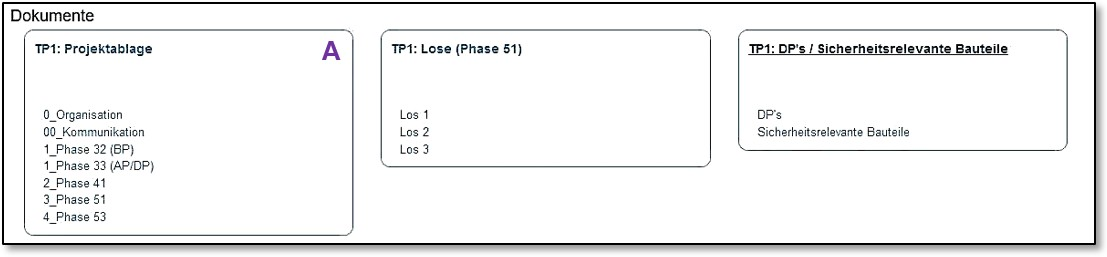
\includegraphics[width=1\linewidth]{../chapters/03_RBS/pictures/01_Dok_Overview_cut.jpg}}
% \caption{Neue Sitzung erfassen}
% \label{fig:speciation}
\end{figure}

Sie können wie gewohnt nach den Tags filtern oder via Navigationsbox die Tags suchen und auswählen \col{(A)}.

Im Bearbeitungsmodus (
\includegraphics[height=12pt]{/Icons/bearbeiten.jpg}) wurde die Handhabung mit den Tags in der Version 2.11 überarbeitet und bietet eine übersichtlichere Auswahl der Tags:

\begin{figure}[H]
\center{
\includegraphics[width=1\linewidth]{../chapters/03_RBS/pictures/02_Dok_Edit_cut.jpg}}
% \caption{Neue Sitzung erfassen}
% \label{fig:speciation}
\end{figure}

Neu finden Sie  den Button 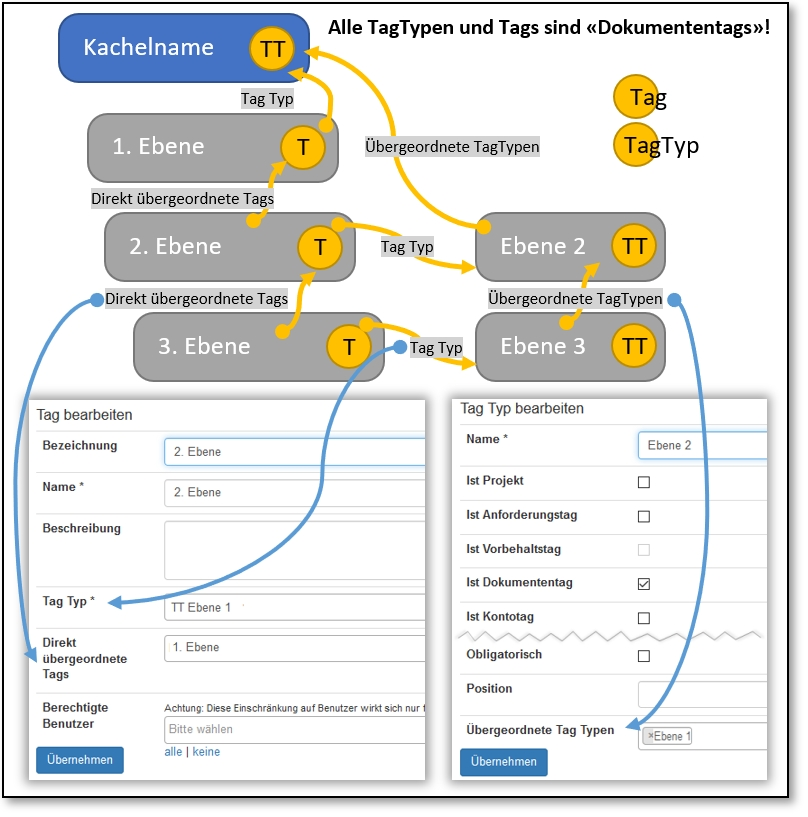
\includegraphics[height=12pt]{/Icons/Tagstruktur.jpg} \col{(B)}, mit welchem Sie direkt die neue Navigation der Tags aufrufen:

% \pagebreak

\begin{wrapfigure}[13]{l}{6.5cm}   % [x] Wie manche Zeile soll sich um die Grafik "brechen"
  \vspace{-23pt}      % Grundwert war 20; mit 30 schön oben beim Text ausgerichtet
  \begin{center}
    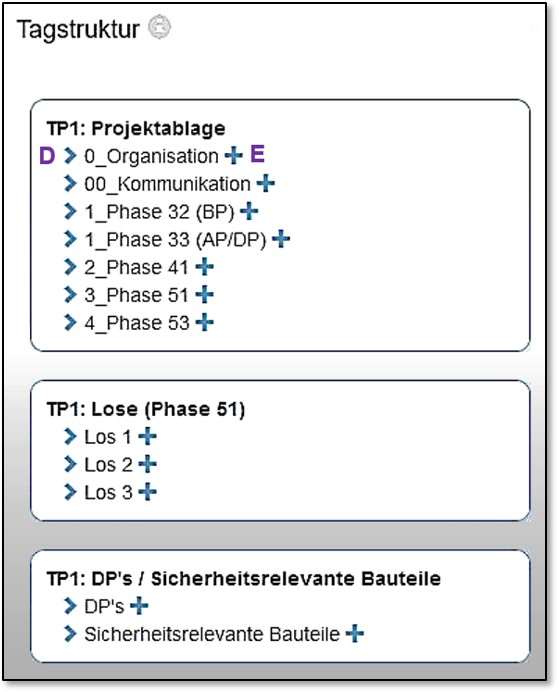
\includegraphics[width=1\linewidth]{../chapters/03_RBS/pictures/04_Dok_Struktur_eingeklappt.jpg}
  \end{center}
  \vspace{-20pt}
%  \caption{Das Menü verwenden}
  \vspace{-10pt}
\end{wrapfigure}

\textbf{Anwendung}: Navigieren Sie mit 
\includegraphics[height=12pt]{/Icons/Pfeil_rechts.jpg} \col{(D)} und klicken Sie hinter dem gesuchten Tag auf das 
\includegraphics[height=12pt]{/Icons/Pluszeichen.jpg}-Zeichen \col{(E)} (Mehrauswahl von Tags ist möglich) und schliessen Sie das Tag-Fenster oben rechts mit 
\includegraphics[height=12pt]{/Icons/X_Button.jpg}. Die Tags wurden im Feld Tags übernommen und können dort auch wieder gelöscht werden.

\vspace{\baselineskip}

\textbf{Hinweis}: Wenn Sie auf der Bearbeitungsseite (
\includegraphics[height=12pt]{/Icons/bearbeiten.jpg}) unter Tags Stichworte eingeben \col{(C)}, wird nach zutreffenden Tags gesucht. Werden diese dort angeklickt, öffnet sich die Tag-Struktur und Sie werden gleich zum ausgewählten Tag geführt. Mit Klick auf das Pluszeichen (
\includegraphics[height=12pt]{/Icons/Pluszeichen.jpg}) wird dieser Tag übernommen. Weitere Tags können angewählt werden. Mit Klick oben rechts im Tag-Fenster (
\includegraphics[height=12pt]{/Icons/X_Button.jpg}) verlassen Sie die Übersicht. Die ausgewählten Tags werden in die Bearbeitungsseite übernommen und können auch wieder gelöscht werden.

\pagebreak
\subsection{Änderungen beim Sitzungswesen:} % Sub-section

\textbf{Globaler Überarbeitungsmodus}:
In der Ansicht 'Protokoll bearbeiten' können Sie den globalen Überarbeitungsmodus ein- und ausschalten. 

\begin{figure}[H]
\center{\includegraphics[width=1\linewidth]{../chapters/03_RBS/pictures/SW_SiBearbeiten_cut.jpg}}
% \caption{Neue Sitzung erfassen}
% \label{fig:speciation}
\end{figure}

Mit einem Klick alle Änderungen bei den Traktandeneinträge annehmen oder ablehnen:

\begin{figure}[H]
\center{\includegraphics[width=1\linewidth]{../chapters/03_RBS/pictures/SW_Ueberarbeiten_cut.jpg}}
% \caption{Neue Sitzung erfassen}
% \label{fig:speciation}
\end{figure}

\textbf{Offene Pendenzen mit einem Klick abrufbar}:
Bei 'Sitzungseinladung bearbeiten' und 'Protokoll bearbeiten' können Sie mittels dem 
\includegraphics[height=12pt]{/Icons/Fahne.jpg}-Icon mit einem Klick direkt auf die offenen Pendenzen wechseln, welche im Zusammenhang mit der Sitzung stehen:

\begin{figure}[H]
\center{\includegraphics[width=1\linewidth]{../chapters/03_RBS/pictures/Pend_Ueb_cut.jpg}}
% \caption{Neue Sitzung erfassen}
% \label{fig:speciation}
\end{figure}

% \vspace{\baselineskip}
% \pagebreak

\textbf{Anhänge bei der Termineinladung und beim Protokoll-Versand}:

Dateien, welche Sie per Link 
\includegraphics[height=12pt]{/Icons/Link.jpg} oder mittels Hochladen 
\includegraphics[height=12pt]{/Icons/Pluszeichen.jpg} an eine Termineinladung oder einem Protokoll angehängt haben, werden bei der Einladung oder beim Protokoll-Versand als Attachment angehängt:

\begin{figure}[H]
\center{\includegraphics[width=1\linewidth]{../chapters/03_RBS/pictures/Anlagen.jpg}}
% \caption{Neue Sitzung erfassen}
% \label{fig:speciation}
\end{figure}

\textbf{Protokollversand}: Sitzungsteilnehmer mit Status 'Eingeladen' stehen im Mailprogramm unter 'An', mit Statuts 'Verteiler' unter 'Cc':

\begin{figure}[H]
\center{\includegraphics[width=1\linewidth]{../chapters/03_RBS/pictures/Versand.jpg}}
% \caption{Neue Sitzung erfassen}
% \label{fig:speciation}
\end{figure}
		
\subsection{Weiterführende Informationen und Support} % Sub-section

Die Detailbeschreibung finden Sie im CUBE PA-Benutzerhandbuch. Für weitere Fragen kontaktieren Sie uns unter {\color{red} cube.support@emchberger.ch}.


\end{document}